\documentclass{article}
\usepackage[utf8]{inputenc}
\usepackage{array}
\usepackage{wrapfig}
\usepackage{multirow}
\usepackage{tabu}
\usepackage{graphicx}
\usepackage{float}
\usepackage{xcolor,colortbl}
\definecolor{green}{rgb}{0.1,0.1,0.1}

\title{Report}
\author{Koray Can Yurtseven}
\date{24.03.2018}

\begin{document}

\maketitle

\section{PART 1}
\subsection{Network 1 Graph}
\begin{figure}[H]
  \caption{Arch1 Sigmoid}
  \centering
  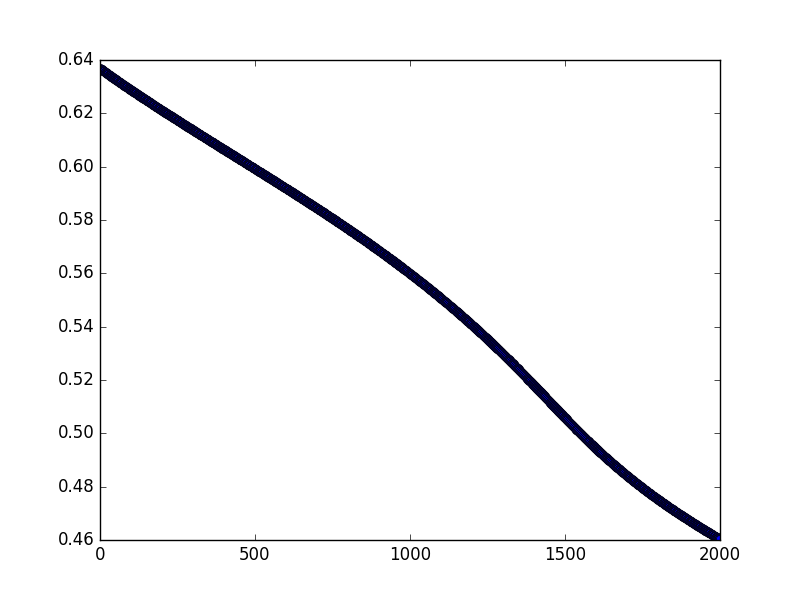
\includegraphics[width=0.8\textwidth]{arch1sigmoid}
\end{figure}
\begin{figure}[H]
  \caption{Arch1 Tanh}
  \centering
  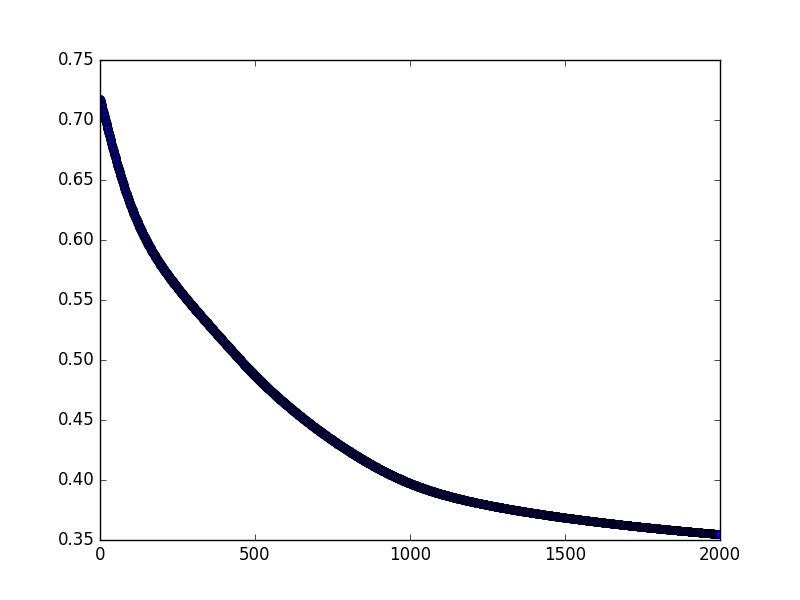
\includegraphics[width=0.8\textwidth]{arch1tanh}
\end{figure}
\begin{figure}[H]
  \caption{Arch1 Relu}
  \centering
  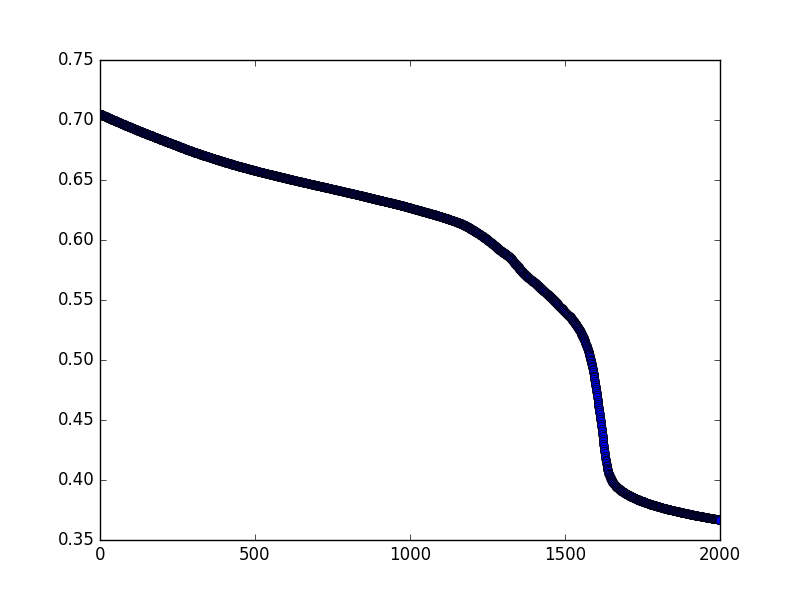
\includegraphics[width=0.8\textwidth]{arch1relu}
\end{figure}
\subsection{Network 2 Graph}
\begin{figure}[H]
  \caption{Arch2 Sigmoid}
  \centering
  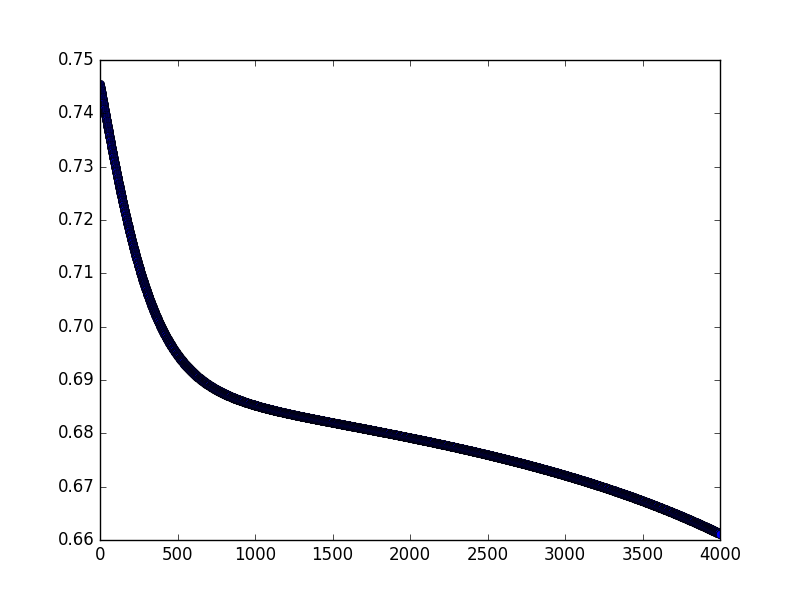
\includegraphics[width=0.8\textwidth]{arch2sigmoid}
\end{figure}
\begin{figure}[H]
  \caption{Arch2 Tanh}
  \centering
  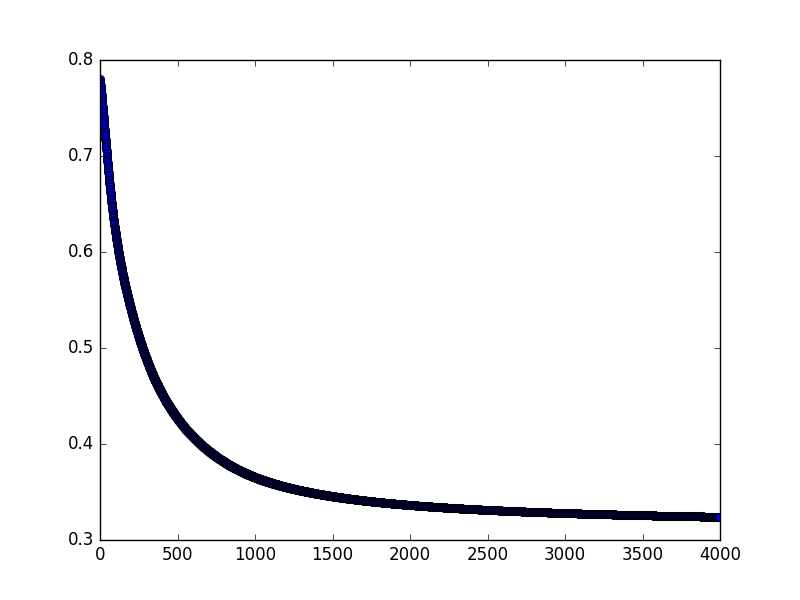
\includegraphics[width=0.8\textwidth]{arch2tanh}
\end{figure}
\begin{figure}[H]
  \caption{Arch2 Relu}
  \centering
  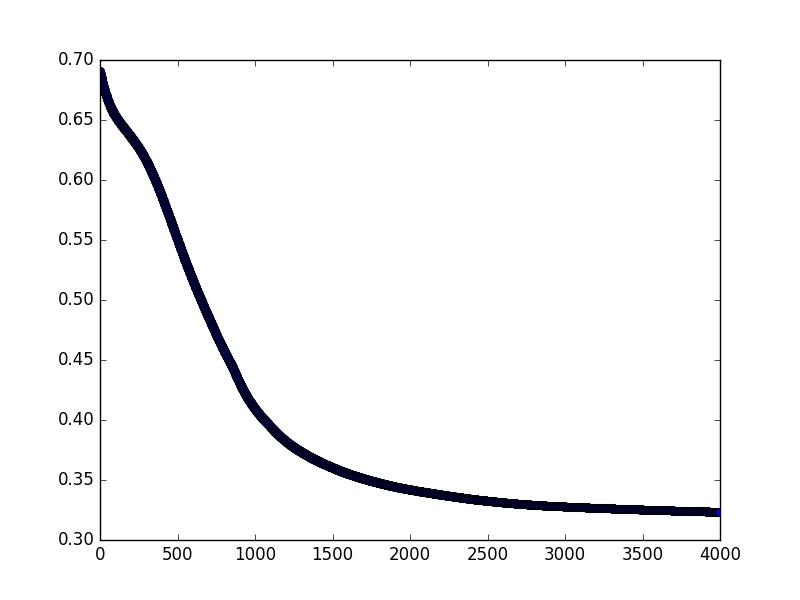
\includegraphics[width=0.8\textwidth]{arch2relu}
\end{figure}
\subsection{Network 3 Graph}
\begin{figure}[H]
  \caption{Arch3 Sigmoid}
  \centering
  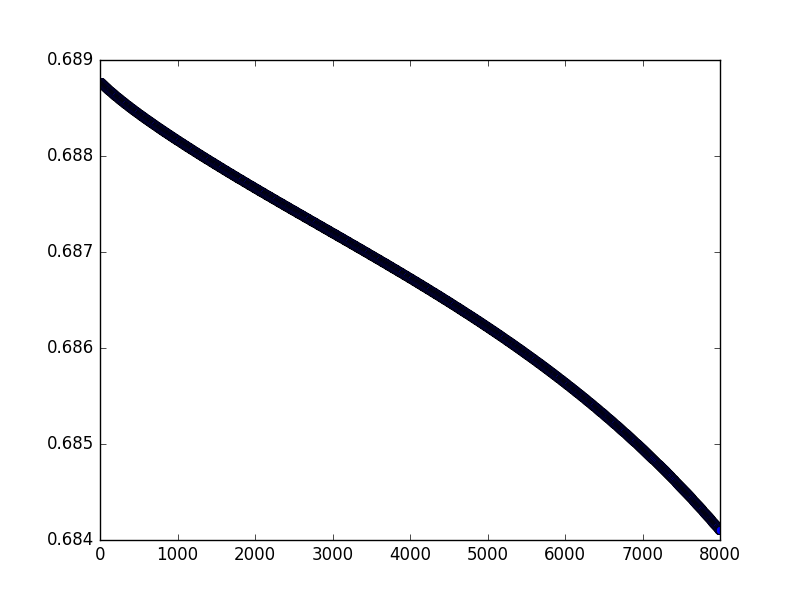
\includegraphics[width=0.8\textwidth]{arch3sigmoid}
\end{figure}
\begin{figure}[H]
  \caption{Arch3 Tanh}
  \centering
  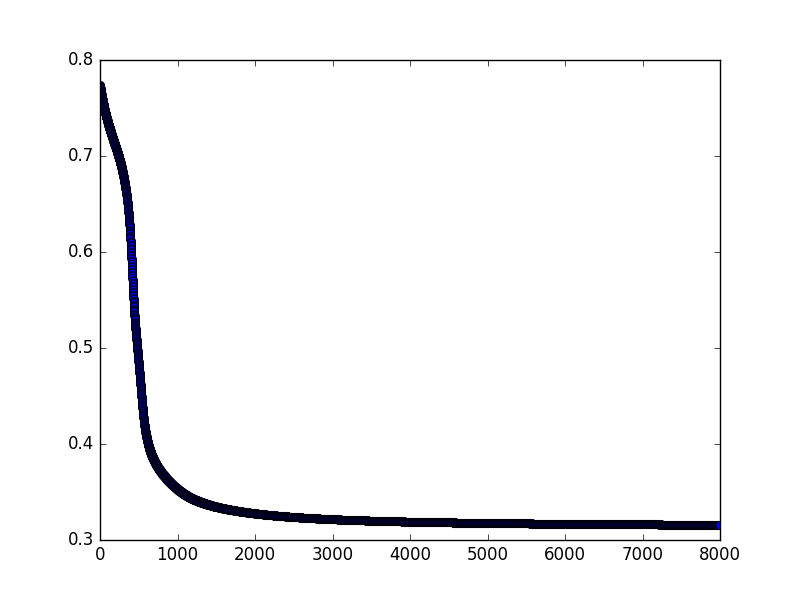
\includegraphics[width=0.8\textwidth]{arch3tanh}
\end{figure}
\begin{figure}[H]
  \caption{Arch3 Relu}
  \centering
  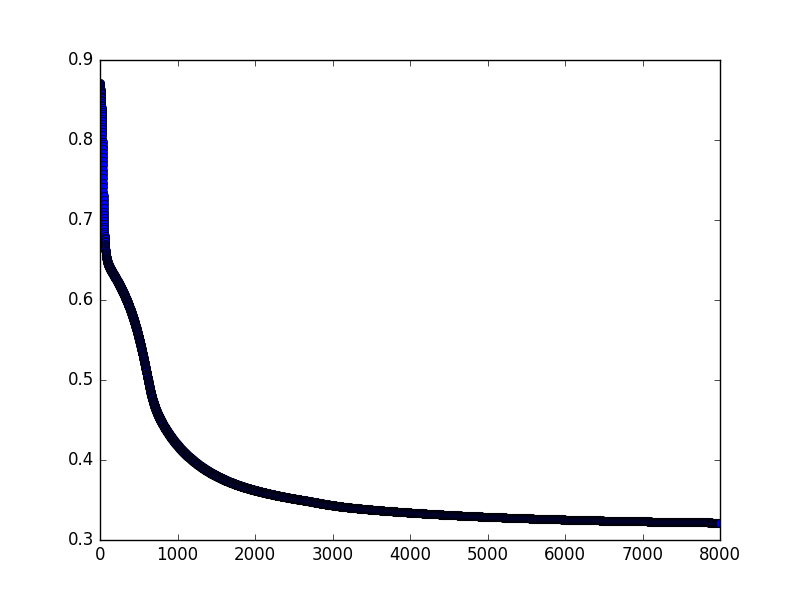
\includegraphics[width=0.8\textwidth]{arch3relu}
\end{figure}

\subsection{Final Accuracy For Each Network}

\begin{table}[H]
\centering
\caption{Final Accuracy For Each Network}
\begin{tabular}{|l|l|l|l|l}
\cline{1-4}
         & Sigmoid    & Tanh      & Relu      &  \\ \cline{1-4}
Network1 & 0.9628821   & 0.99126637 & 0.9737991 &  \\ \cline{1-4}
Network2 & 0.55458516 & 1.0       & 0.9956332  &  \\ \cline{1-4}
Network3 & 0.55458516  & 1.0       & 1.0 &  \\ \cline{1-4}
\end{tabular}
\end{table}

\subsection{Hyperparameter Optimization}
\subsubsection{Optimization}
In the table, xx/yy denotes that:
xx is loss value, yy is accuracy rating for epoch at 2000, then testing the data.
\begin{table}[H]
    \resizebox{\columnwidth}{!}{%
    \centering
    \begin{tabular}{|c|c|c|c|c|c|c|c|c|c|c|}
    \hline
    \multirow{2}{5em}{Layer Activations} & \multicolumn{10}{c|}{Learning Rate} \\
        & 0.01 & 0.02 & 0.03 & 0.04 & 0.05 & 0.06 & 0.07 & 0.08 & 0.09 & 0.1 \\
        \hline \hline
        SSS & 0.68789244/0.55 & 
0.6692991/0.55 & 
0.66720015/0.55 & 
0.68628144/0.55 & 
0.6810556/0.55 & 
0.47050172/0.97 & 
0.6871969/0.55 & 
0.3463915/0.99 & 
0.33197898/0.99 & 
 \cellcolor{blue!25} 0.33075026/0.99  \\
        \hline
        SST & 0.4378503/0.98 & 
0.43045545/0.96 & 
0.38875714/0.98 & 
0.32834312/1.0 & 
0.32441178/1.0 & 
0.319201/1.0 & 
0.3197482/1.0 & 
0.31692475/1.0 & 
\cellcolor{blue!25} 0.3160016/1.0 & 
0.3175097/1.0  \\
        \hline
        SSR & 0.6850313/0.55 & 
0.38780826/0.99 & 
0.34500504/1.0 & 
0.34083718/0.99 & 
0.32920367/1.0 & 
0.6869073/0.55 & 
0.3213476/1.0 & 
0.327354/1.0 & 
\cellcolor{blue!25} 0.317619/1.0 & 
0.32001895/1.0  \\
        \hline
        STS & 0.6145127/0.74 & 
0.36037236/0.99 & 
0.34948123/0.99 & 
0.4112389/0.99 & 
0.32826188/1.0 & 
0.32640412/1.0 & 
0.32546172/1.0 & 
0.32089263/1.0 & 
\cellcolor{blue!25} 0.32020745/1.0 & 
0.32081103/1.0  \\
        \hline
        STT & 0.35425475/0.99 & 
0.32510495/1.0 & 
0.31968254/1.0 & 
0.317732/1.0 & 
0.31772736/1.0 & 
0.31646454/1.0 & 
0.3150846/1.0 & 
0.31529894/1.0 & 
0.31494474/1.0 & 
\cellcolor{blue!25} 0.31449395/1.0 \\
        \hline
        STR & 0.44032148/0.98 & 
0.3497323/1.0 & 
0.33083186/1.0 & 
0.33689547/1.0 & 
0.31755918/1.0 & 
0.31503657/1.0 & 
0.31482077/1.0 & 
0.31454292/1.0 & 
0.31412834/1.0 & 
\cellcolor{blue!25} 0.3140219/1.0  \\
        \hline
        SRS & 0.6634242/0.70 & 
0.40922305/0.99 & 
0.39515218/0.99 & 
0.39538285/0.99 & 
0.6546068/0.72 & 
0.33624896/0.99 & 
0.32252526/1.0 & 
\cellcolor{blue!25} 0.3191166/1.0 & 
0.32551947/1.0 & 
0.32132214/1.0  \\
        \hline
        SRT & 0.48628902/0.87 & 
0.32630733/1.0 & 
0.32008824/1.0 & 
0.32077998/1.0 & 
0.31678194/1.0 & 
0.316255/1.0 & 
0.3157316/1.0 & 
0.31525585/1.0 & 
\cellcolor{blue!25} 0.3150004/1.0 & 
0.3151544/1.0  \\
        \hline
        SRR & 0.6603494/0.62 & 
0.34231156/0.99 & 
0.33227438/1.0 & 
0.31815103/1.0 & 
0.3214322/1.0 & 
0.32806572/1.0 & 
0.32187757/1.0 & 
\cellcolor{blue!25} 0.3145783/1.0 & 
0.31480974/1.0 & 
0.31693384/1.0  \\
        \hline
        TSS & 0.6843663/0.55 & 
0.67058444/0.55 & 
0.6176693/0.80 & 
0.62599444/0.56 & 
0.36207137/0.99 & 
0.35972127/0.99 & 
0.34869736/0.99 & 
0.34090057/0.99 & 
0.3292783/1.0 & 
\cellcolor{blue!25} 0.3251485/1.0  \\
        \hline
        TST & 0.48351938/0.98 & 
0.3431558/0.99 & 
0.32776284/0.99 & 
0.3188361/1.0 & 
0.31751505/1.0 & 
0.3167492/1.0 & 
0.31694236/1.0 & 
0.31781915/1.0 & 
0.31579846/1.0 & 
\cellcolor{blue!25} 0.31513965/1.0  \\
        \hline
        TSR & 0.4043094/0.98 & 
0.33192244/0.99 & 
0.40323663/0.99 & 
0.3286709/1.0 & 
0.3238838/1.0 & 
0.32062533/1.0 & 
0.31532422/1.0 & 
0.3156018/1.0 & 
0.31660658/1.0 & 
\cellcolor{blue!25} 0.31425402/1.0  \\
        \hline
        TTS & 0.5588452/0.89 & 
0.34751627/0.99 & 
0.33776295/1.0 & 
0.3259682/1.0 & 
0.32522935/1.0 & 
0.32212046/1.0 & 
0.33072641/1.0 & 
0.31895778/1.0 & 
0.31818497/1.0 & 
\cellcolor{blue!25} 0.31753024/1.0  \\
        \hline
        TTT & 0.33037642/1.0 & 
0.3198712/1.0 & 
0.31743637/1.0 & 
0.31665117/1.0 & 
0.31565586/1.0 & 
0.31516674/1.0 & 
0.3150601/1.0 & 
0.31431255/1.0 & 
0.3143746/1.0 & 
\cellcolor{blue!25} 0.31425974/1.0 \\
        \hline
        TTR & 0.571504/0.77 & 
0.3187649/1.0 & 
0.31588382/1.0 & 
0.315084/1.0 & 
0.32032195/1.0 & 
0.31422964/1.0 & 
0.31633186/1.0 & 
0.31378192/1.0 & 
0.31392214/1.0 & 
\cellcolor{blue!25} 0.31360024/1.0  \\
        \hline
        TRS & 0.52846014/0.91 & 
0.3693901/0.98 & 
0.33349907/1.0 & 
0.33436558/1.0 & 
0.3267495/1.0 & 
0.32285532/1.0 & 
0.32632208/1.0 & 
0.31937024/1.0 & 
0.3235086/1.0 & 
\cellcolor{blue!25} 0.31890053/1.0  \\
        \hline
        TRT & 0.3400546/1.0 & 
0.32522988/1.0 & 
0.32008892/1.0 & 
0.3192825/0.99 & 
0.31575373/1.0 & 
0.31488732/1.0 & 
0.31489557/1.0 & 
0.31482056/1.0 & 
\cellcolor{blue!25} 0.3146442/1.0 & 
0.315066/1.0  \\
        \hline
        TRR & 0.340073/1.0 & 
0.33295488/1.0 & 
0.3248766/1.0 & 
0.32158422/1.0 & 
0.32000777/1.0 & 
\cellcolor{blue!25} 0.31396133/1.0 & 
0.31835827/1.0 & 
0.314066/1.0 & 
0.31669813/1.0 & 
0.3163897/1.0  \\
        \hline
        RSS & 0.67796135/0.55 & 
0.6737318/0.55 & 
0.4599986/0.98 & 
0.3500972/1.0 & 
0.33876064/1.0 & 
0.34116995/0.99 & 
0.33178085/1.0 & 
0.33159533/1.0 & 
0.325827/1.0 & 
\cellcolor{blue!25} 0.32536262/1.0  \\
        \hline
        RST & 0.515099/0.93 & 
0.33028436/1.0 & 
0.32511172/1.0 & 
0.31738698/1.0 & 
0.31828427/1.0 & 
0.3164119/1.0 & 
0.31586108/1.0 & 
0.3151228/1.0 & 
\cellcolor{blue!25} 0.3146528/1.0 & 
0.31483337/1.0  \\
        \hline
        RSR & 0.41590893/0.99 & 
0.32236278/1.0 & 
0.31979418/1.0 & 
0.31712398/1.0 & 
0.31540766/1.0 & 
0.31509206/1.0 & 
0.31484774/1.0 & 
\cellcolor{blue!25} 0.31456298/1.0 & 
0.31730348/1.0 & 
0.31758767/1.0  \\
        \hline
        RTS & 0.5438701/0.88 & 
0.3819605/0.99 & 
0.33970806/1.0 & 
0.32761222/1.0 & 
0.32699257/1.0 & 
0.3231281/1.0 & 
0.31967098/1.0 & 
0.31935352/1.0 & 
0.3177113/1.0 & 
\cellcolor{blue!25} 0.31755465/1.0  \\
        \hline
        RTT & 0.33895338/0.99 & 
0.32027683/1.0 & 
0.31740025/1.0 & 
0.31562498/1.0 & 
0.31539953/1.0 & 
0.31515348/1.0 & 
0.31465614/1.0 & 
0.31485334/1.0 & 
0.31440407/1.0 & 
\cellcolor{blue!25} 0.3142189/1.0  \\
        \hline
        RTR & 0.3678897/0.99 & 
0.3307278/1.0 & 
0.32895288/1.0 & 
0.31448418/1.0 & 
0.31420946/1.0 & 
0.3140565/1.0 & 
0.31419283/1.0 & 
0.31376797/1.0 & 
0.3155947/1.0 & 
\cellcolor{blue!25} 0.3136963/1.0  \\
        \hline
        RRS & 0.45061308/0.99 & 
0.36469537/1.0 & 
0.34686592/1.0 & 
0.32555684/1.0 & 
0.32504523/1.0 & 
0.31998438/1.0 & 
0.32159403/1.0 & 
0.32045943/1.0 & 
0.31848156/1.0 & 
\cellcolor{blue!25} 0.31729102/1.0 \\
        \hline
        RRT & 0.3257437/0.99 & 
0.329249/0.99 & 
0.31823364/1.0 & 
0.31600565/1.0 & 
0.31527776/1.0 & 
0.31876868/0.99 & 
0.31521088/1.0 & 
0.31437874/1.0 & 
\cellcolor{blue!25} 0.31411266/1.0 & 
0.31420094/1.0  \\
        \hline
        RRR & 0.3644881/0.99 & 
0.3174078/1.0 & 
0.31480208/1.0 & 
0.31403202/1.0 & 
0.31995615/1.0 & 
0.31404272/1.0 & 
0.31381625/1.0 & 
\cellcolor{blue!25} 0.31364825/1.0 & 
0.31408548/1.0 & 
0.31622016/1.0 \\
        \hline
        
\end{tabular}%
}
\end{table}

where S is \verb|sigmoid|, T is \verb|tanh| and R is \verb|relu| activation function. For highlighting, I look at the loss and accuracy values of architectures and colored the lowest value of loss and highest value of accuracy. In all 27 architecture, the best values have 1.0 accuracy. In architecture TTR, with 0.1 learning rate, my loss value is the lowest and therefore I choose that architecture to part below.
\subsubsection{Training and Test}

Accuracy is 1.0

\begin{figure}[H]
  \caption{Arch3 Optimized, Rate= 0.1, TTR}
  \centering
  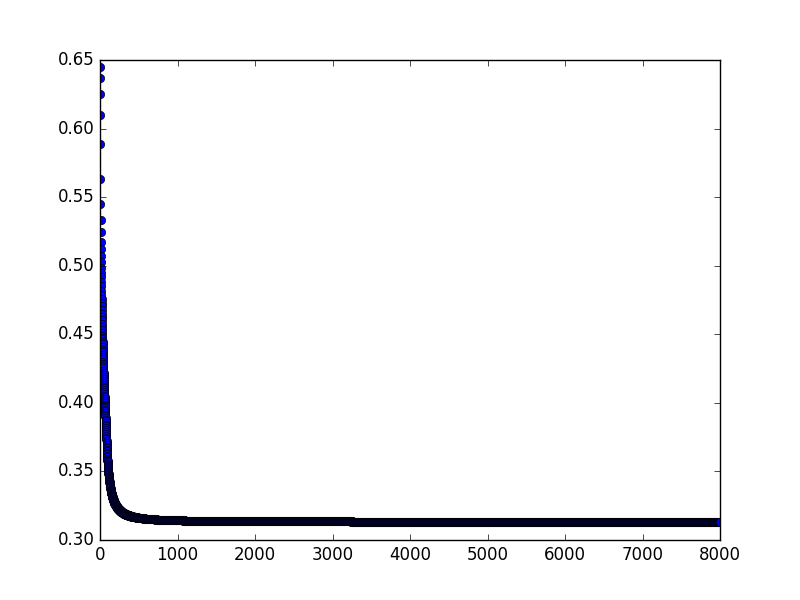
\includegraphics[width=0.8\textwidth]{arch3opt}
\end{figure}

\section{PART 2}

\begin{figure}[H]
  \caption{Part 2}
  \centering
  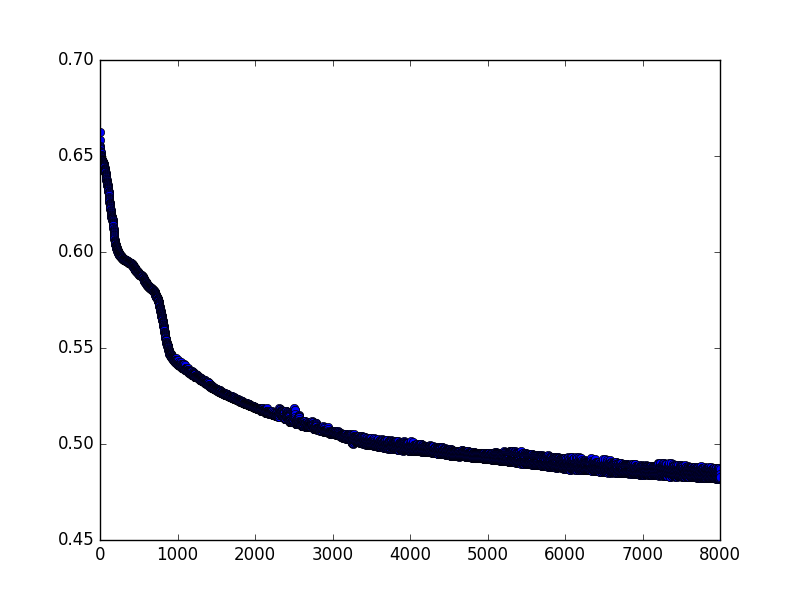
\includegraphics[width=0.8\textwidth]{part2}
\end{figure}

I've used same architecture in previous parts. Every time I change the units in the layer, I have different results. RRR architecture with 8000 training gave my best result among others. I've used 0.07 rating rate and  obtain 0.83 accuracy rating with the given set.
\end{document}
